\section{Constructing Cartesian Coordinates from Euclidean Geometry}

We begin with a Euclidean plane, not with ordered pairs. Points, straight
lines, perpendicularity, congruent segments, segment bisection, and the
Pythagorean theorem are assumed to be available before coordinates are
introduced. Cartesian coordinates will provide numerical labels for this
existing geometry.

\begin{remarkbox}
Coordinates do not create Euclidean geometry. They encode it.
\end{remarkbox}

\subsection{The Plane Before Coordinates}

At first there is no distinguished origin, no preferred direction, and no
numerical scale.

\begin{center}
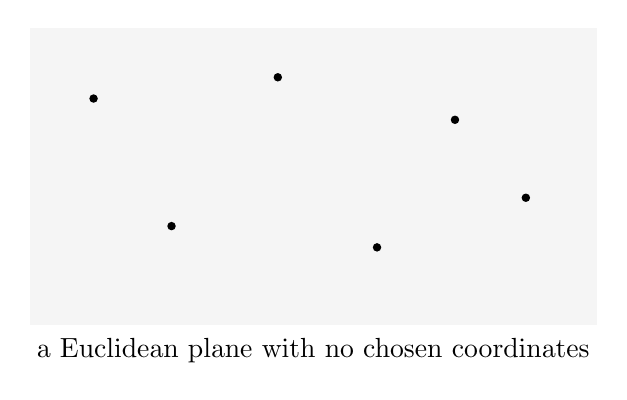
\begin{tikzpicture}[scale=0.9]
    \fill[gray!8] (-4,-2.1) rectangle (4,2.1);
    \foreach \x/\y in {-3.1/1.1,-2.0/-0.7,-0.5/1.4,0.9/-1.0,2.0/0.8,3.0/-0.3} {
        \fill (\x,\y) circle (1.7pt);
    }
    \node at (0,-2.45) {a Euclidean plane with no chosen coordinates};
\end{tikzpicture}
\end{center}

\begin{definitionbox}
For the construction below we use the following Euclidean operations:
\begin{itemize}
    \item drawing the line through two distinct points;
    \item constructing a perpendicular through a point;
    \item transferring a segment length with a compass;
    \item bisecting a segment;
    \item applying the Pythagorean theorem.
\end{itemize}
\end{definitionbox}

\subsection{Choosing the Axes and the Origin}

Choose a line and a point $O$ on it. The line will become the $x$-axis and
$O$ will become the origin. Through $O$, construct the line perpendicular to
the first one. This becomes the $y$-axis.

\begin{center}
\begin{tikzpicture}[scale=0.9]
    \draw[axis] (-4.2,0) -- (4.4,0) node[right] {$x$};
    \draw[axis] (0,-3.1) -- (0,3.3) node[above] {$y$};
    \fill (0,0) circle (2pt);
    \node[below left] at (0,0) {$O$};
    \draw (0.26,0) -- (0.26,0.26) -- (0,0.26);
\end{tikzpicture}
\end{center}

The axes are perpendicular because this was required in their geometric
construction. No coordinate formula has yet been used.

\subsection{Choosing a Common Unit}

Choose a positive length and call it one unit. Transfer the same length with a
compass along both axes and in both directions. Repetition gives the integer
marks.

\begin{center}
\begin{tikzpicture}[scale=0.9]
    \draw[axis] (-4.2,0) -- (4.4,0) node[right] {$x$};
    \draw[axis] (0,-3.1) -- (0,3.3) node[above] {$y$};
    \foreach \x in {-3,-2,-1,1,2,3} {
        \draw (\x,0.09) -- (\x,-0.09) node[below=3pt] {$\x$};
    }
    \foreach \y in {-2,-1,1,2} {
        \draw (0.09,\y) -- (-0.09,\y) node[left=3pt] {$\y$};
    }
    \node[below left] at (0,0) {$0$};
    \draw[<->,gray] (0,2.65) -- (1,2.65) node[midway,above] {one unit};
\end{tikzpicture}
\end{center}

\begin{remarkbox}
Using one common unit on both axes is essential. It makes a horizontal unit
congruent to a vertical unit.
\end{remarkbox}

\subsection{Refining the Scale}

Bisecting a unit segment gives halves; repeating the construction gives
quarters, eighths, and in general the dyadic marks
\[
\frac{k}{2^n},
\qquad k\in\mathbb Z,
\quad n\in\mathbb N.
\]

\begin{center}
\begin{tikzpicture}[scale=1.1]
    \draw[axis] (-0.4,0) -- (4.4,0);
    \foreach \x/\lab in {0/0,1/{\frac14},2/{\frac12},3/{\frac34},4/1} {
        \draw (\x,0.1) -- (\x,-0.1) node[below=4pt] {$\lab$};
    }
    \node[above] at (2,0.35) {successive bisections};
\end{tikzpicture}
\end{center}

These marks approximate every axis position arbitrarily closely. Identifying
all positions exactly with real numbers uses the usual continuity and
completeness assumptions of Euclidean measurement.

\subsection{Assigning Coordinates by Orthogonal Projection}

Let $P$ be a point of the plane. Through $P$, draw a line perpendicular to the
$x$-axis and let its intersection with the axis be $P_x$. Similarly construct
$P_y$ on the $y$-axis.

\begin{center}
\begin{tikzpicture}[scale=0.9]
    \draw[axis] (-1.1,0) -- (5.0,0) node[right] {$x$};
    \draw[axis] (0,-1.1) -- (0,4.0) node[above] {$y$};
    \coordinate (P) at (3.2,2.4);
    \coordinate (Px) at (3.2,0);
    \coordinate (Py) at (0,2.4);
    \draw[helper] (P) -- (Px);
    \draw[helper] (P) -- (Py);
    \fill (P) circle (2.2pt) node[above right] {$P$};
    \fill (Px) circle (1.8pt) node[below] {$P_x$};
    \fill (Py) circle (1.8pt) node[left] {$P_y$};
\end{tikzpicture}
\end{center}

If the signed labels of $P_x$ and $P_y$ are $x$ and $y$, respectively, then
we assign to $P$ the ordered pair
\[
P\longleftrightarrow(x,y).
\]

\begin{theorembox}
Once the perpendicular axes, their positive directions, and a common unit are
fixed, every point of the plane has exactly one coordinate pair and every pair
$(x,y)\in\mathbb R^2$ determines exactly one point. Hence
\[
\boxed{
\text{points of the Euclidean plane}
\longleftrightarrow
\text{pairs }(x,y)\in\mathbb R^2
}.
\]
\end{theorembox}

\subsection{The Distance Formula}

For points
\[
P=(x_1,y_1),
\qquad
Q=(x_2,y_2),
\]
the horizontal and vertical separations are
\[
|x_2-x_1|
\qquad\text{and}\qquad
|y_2-y_1|.
\]
They form the legs of a right triangle whose hypotenuse is $PQ$.

\begin{center}
\begin{tikzpicture}[scale=0.9]
    \draw[axis] (-0.8,0) -- (5.2,0) node[right] {$x$};
    \draw[axis] (0,-0.8) -- (0,4.5) node[above] {$y$};
    \coordinate (P) at (1,1);
    \coordinate (Q) at (4,3.5);
    \coordinate (R) at (4,1);
    \draw[subset] (P) -- (Q);
    \draw[helper] (P) -- (R) node[midway,below] {$|x_2-x_1|$};
    \draw[helper] (R) -- (Q) node[midway,right] {$|y_2-y_1|$};
    \draw (3.72,1) -- (3.72,1.28) -- (4,1.28);
    \fill (P) circle (2pt) node[below left] {$P$};
    \fill (Q) circle (2pt) node[above right] {$Q$};
\end{tikzpicture}
\end{center}

By the Pythagorean theorem,
\[
d_E(P,Q)^2
=
(x_2-x_1)^2+(y_2-y_1)^2,
\]
so
\[
\boxed{
d_E(P,Q)
=
\sqrt{(x_2-x_1)^2+(y_2-y_1)^2}
}.
\]

\subsection{Angles and Their Measure}

Only now, after the coordinate construction and the distance formula are in
place, do we record how angles are understood in the Euclidean plane.

\begin{definitionbox}
An angle with vertex $O$ is the part of the plane determined by two rays with
common initial point $O$, together with the choice of which of the two regions
between the rays is meant.
\end{definitionbox}

The angle is a geometric object. Its measure is a number assigned by comparing
that region with a full turn about the vertex.

\begin{definitionbox}
A full turn is assigned the measure
\[
360^\circ.
\]
If an angle occupies the fraction $r$ of a full turn, then its degree measure is
\[
m(\alpha)=360^\circ r.
\]
\end{definitionbox}

Therefore a half-turn has measure
\[
180^\circ,
\]
and one quarter of a full turn has measure
\[
90^\circ.
\]

\begin{center}
\begin{tikzpicture}[scale=1.0]
    \coordinate (O) at (0,0);
    \draw[axis] (O) -- (3.4,0) node[right] {$r_1$};
    \draw[axis] (O) -- (0,3.0) node[above] {$r_2$};
    \draw[subset] (1.0,0) arc[start angle=0,end angle=90,radius=1.0];
    \node[subset label] at (0.72,0.72) {$90^\circ$};
    \fill (O) circle (2pt) node[below left] {$O$};
    \draw (0.28,0) -- (0.28,0.28) -- (0,0.28);
\end{tikzpicture}
\end{center}

\begin{theorembox}
Two perpendicular lines through a point divide a full turn into four congruent
angles. Hence each of them has measure
\[
\frac{360^\circ}{4}=90^\circ.
\]
Such an angle is called a right angle.
\end{theorembox}

The coordinate axes were chosen to be perpendicular before coordinates were
assigned. The statement that they form a right angle is therefore inherited
from the Euclidean construction, not created by an algebraic formula.

\begin{remarkbox}
The same angle may later be measured in radians. A full turn is $2\pi$ radians,
so
\[
90^\circ=\frac{\pi}{2}.
\]
Degrees and radians are two numerical scales for the same Euclidean angle.
\end{remarkbox}

\begin{summarybox}
The construction proceeds in the following order:
\begin{enumerate}
    \item start with a Euclidean plane;
    \item choose perpendicular axes, positive directions, and a common unit;
    \item refine the scale and identify axis positions with real numbers;
    \item assign coordinates by orthogonal projection;
    \item derive the distance formula from the Pythagorean theorem;
    \item finally describe angles and their numerical measure.
\end{enumerate}
Coordinates are a numerical representation of the original Euclidean geometry.
\end{summarybox}
